\documentclass{article}
\usepackage[utf8]{inputenc}
\usepackage{amsfonts}
\usepackage{algorithm2e}
\usepackage{amsmath}
\usepackage[a4paper]{geometry}
\geometry{hscale=0.8,vscale=0.9,centering}
\usepackage{graphicx}
\usepackage{program}
\usepackage{ulem}
\usepackage{xcolor}
\usepackage{pdfpages}

\title{M1 Info – ARC - LAB2}
\author{Olivier HUREAU }
\date{18/03/2020}

\begin{document}
\maketitle

\section{Dessin de l'automate}

\begin{figure}[!h]
\advance\leftskip+3.5cm
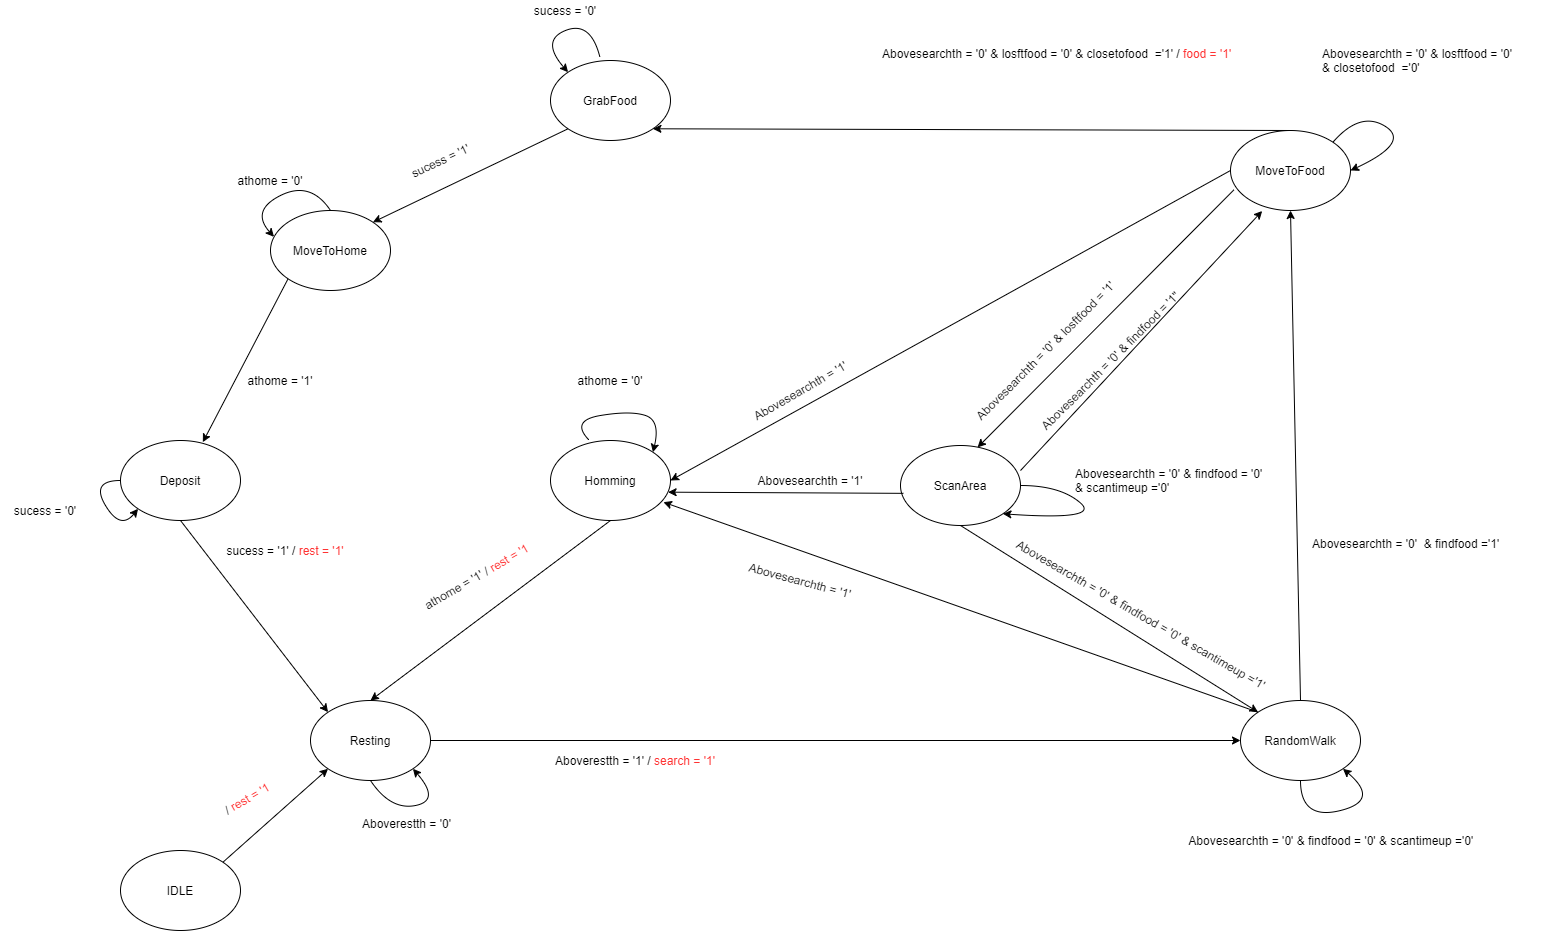
\includegraphics[scale=0.36, angle=-90]{Automate.png}
\caption{Automate du robot}
\end{figure}

\newpage
\section{Description VHDL comportementale}
Le code source est donné en annexe du document (robot.vhd et testRobot.vhd)

\section{TestRobot}
\subsection{Réalisation du test}
Pour tester mon implémentation, j'ai tout d'abord rédigé un tableau des différentes entrées et sorties et des comportements que ceux-ci devais avoir pour toutes les transitions ainsi que les différentes pour y accéder depuis un reset de l'automate.

Dans ce tableau se trouve différentes informations tel que : En rouge :  les inputs que je doit mettre à 1, En bleu : les données que doivent prendre les outputs. 

Ce tableau est fournis en annexe. 
\subsection{Interpretation du test}

Après simulation, on obtiens les différents graphes fournis en annexe. La figure 2 représente la totalité de la simulation. Les figures 3, 4 et 5 sont cette même simulation partitionné. 

Ce que l'on peux observer avec ces différents graphes c'est que notre simulation implémente bien le problème. Les sorties  et la suite d'état correspondent bien à ce qui a était prédit dans notre tableau.

\section{Counter}
Le code source est donné en annexe du document (count.vhd et testCount.vhd)

Après simulation, sur la figure 6 on observe bien que le compteur ne se met en marche uniquement lorsque l'état start est à 1 et le reset fonctionne bien. Le nombre de front montant compté est le bon.



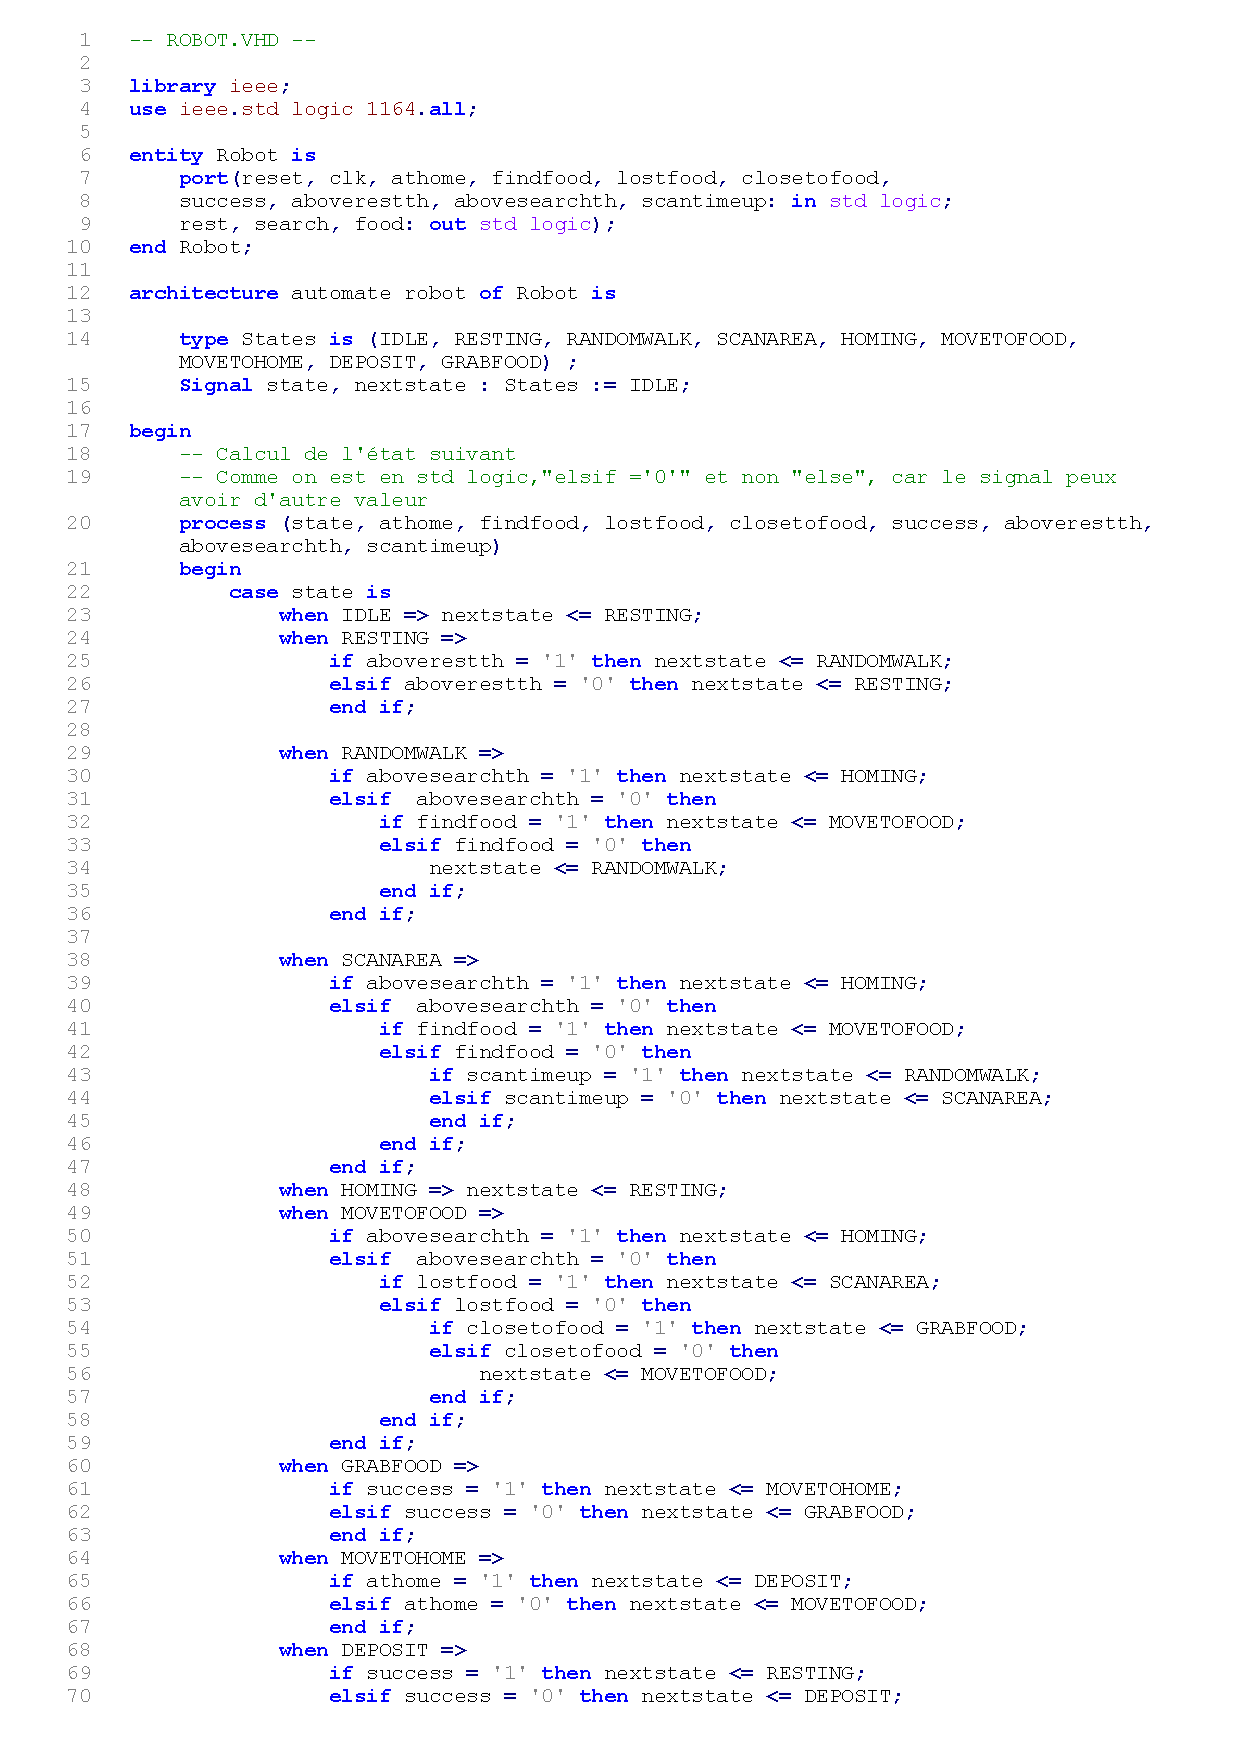
\includepdf{robot.pdf}
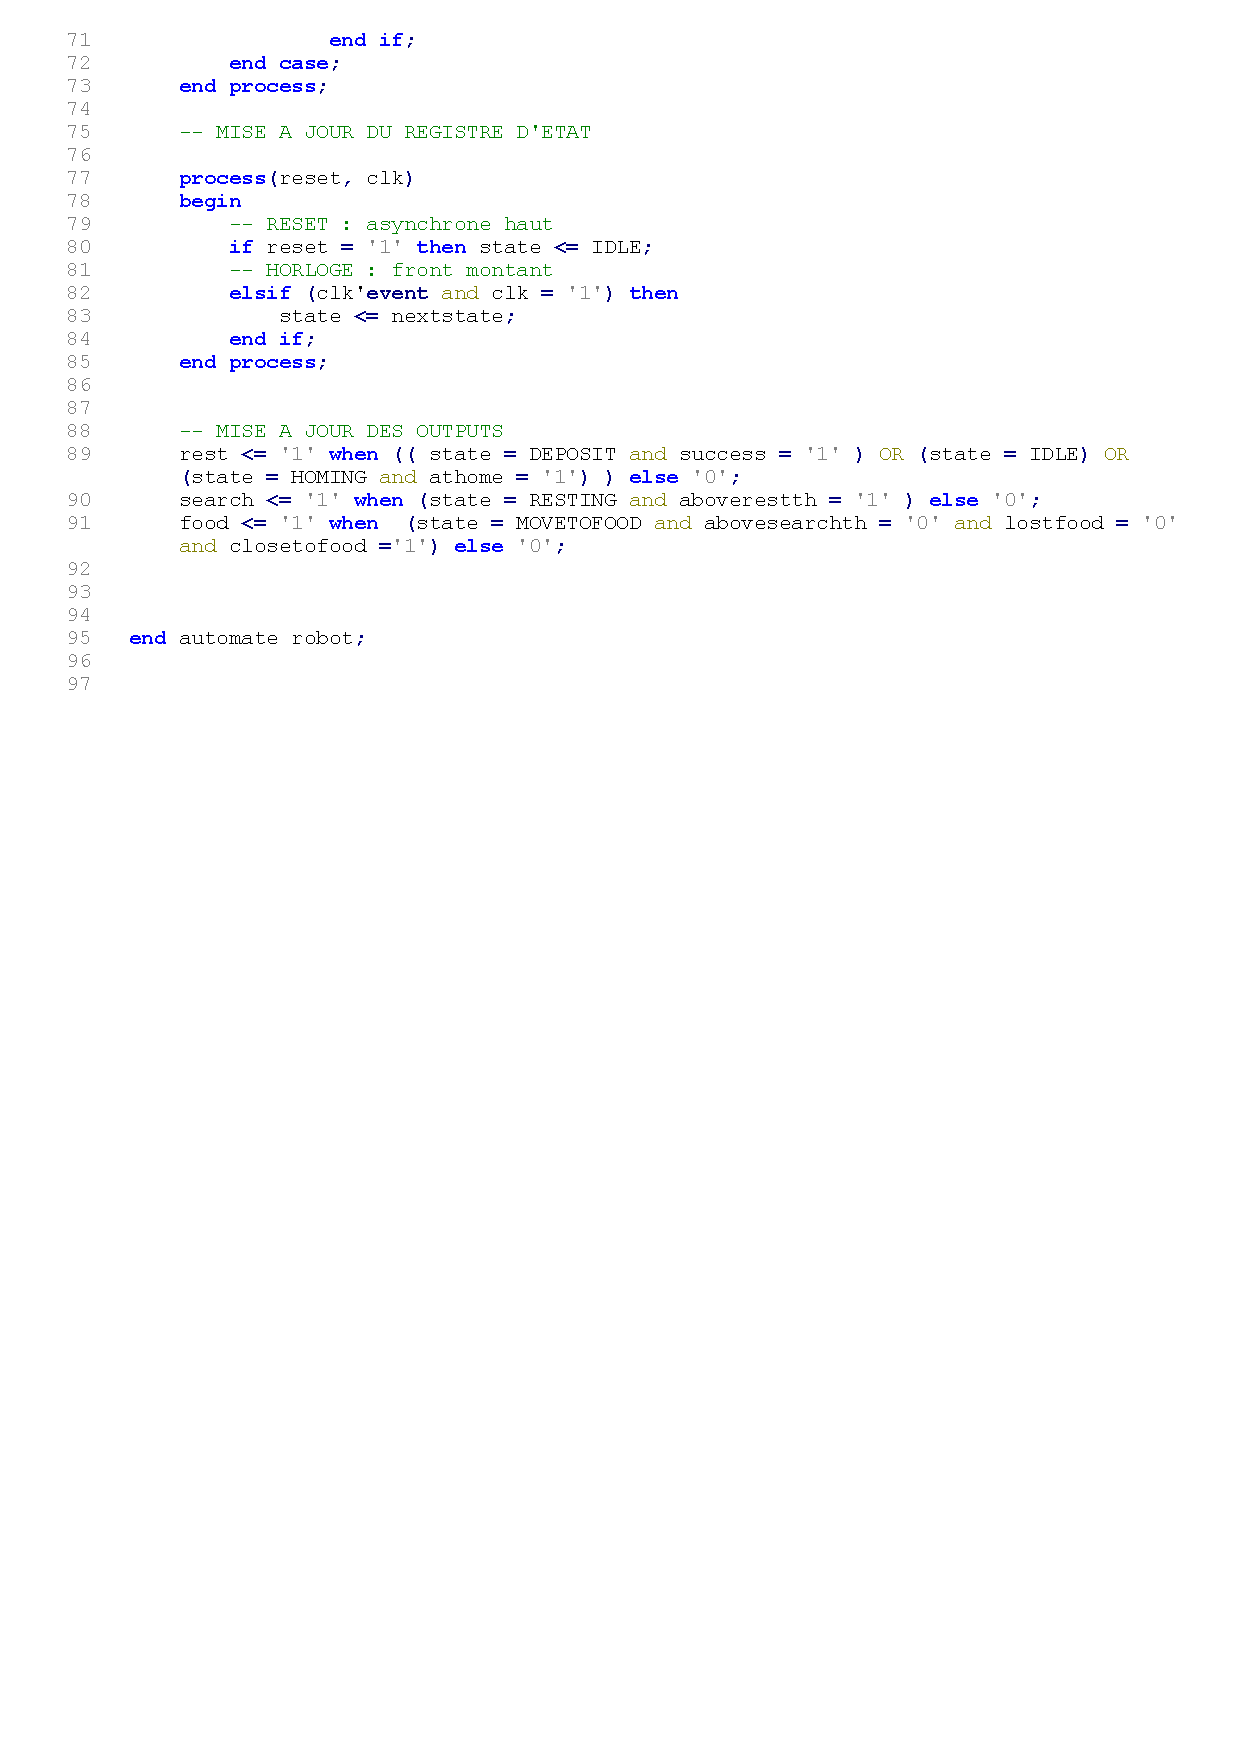
\includepdf{robot2.pdf}
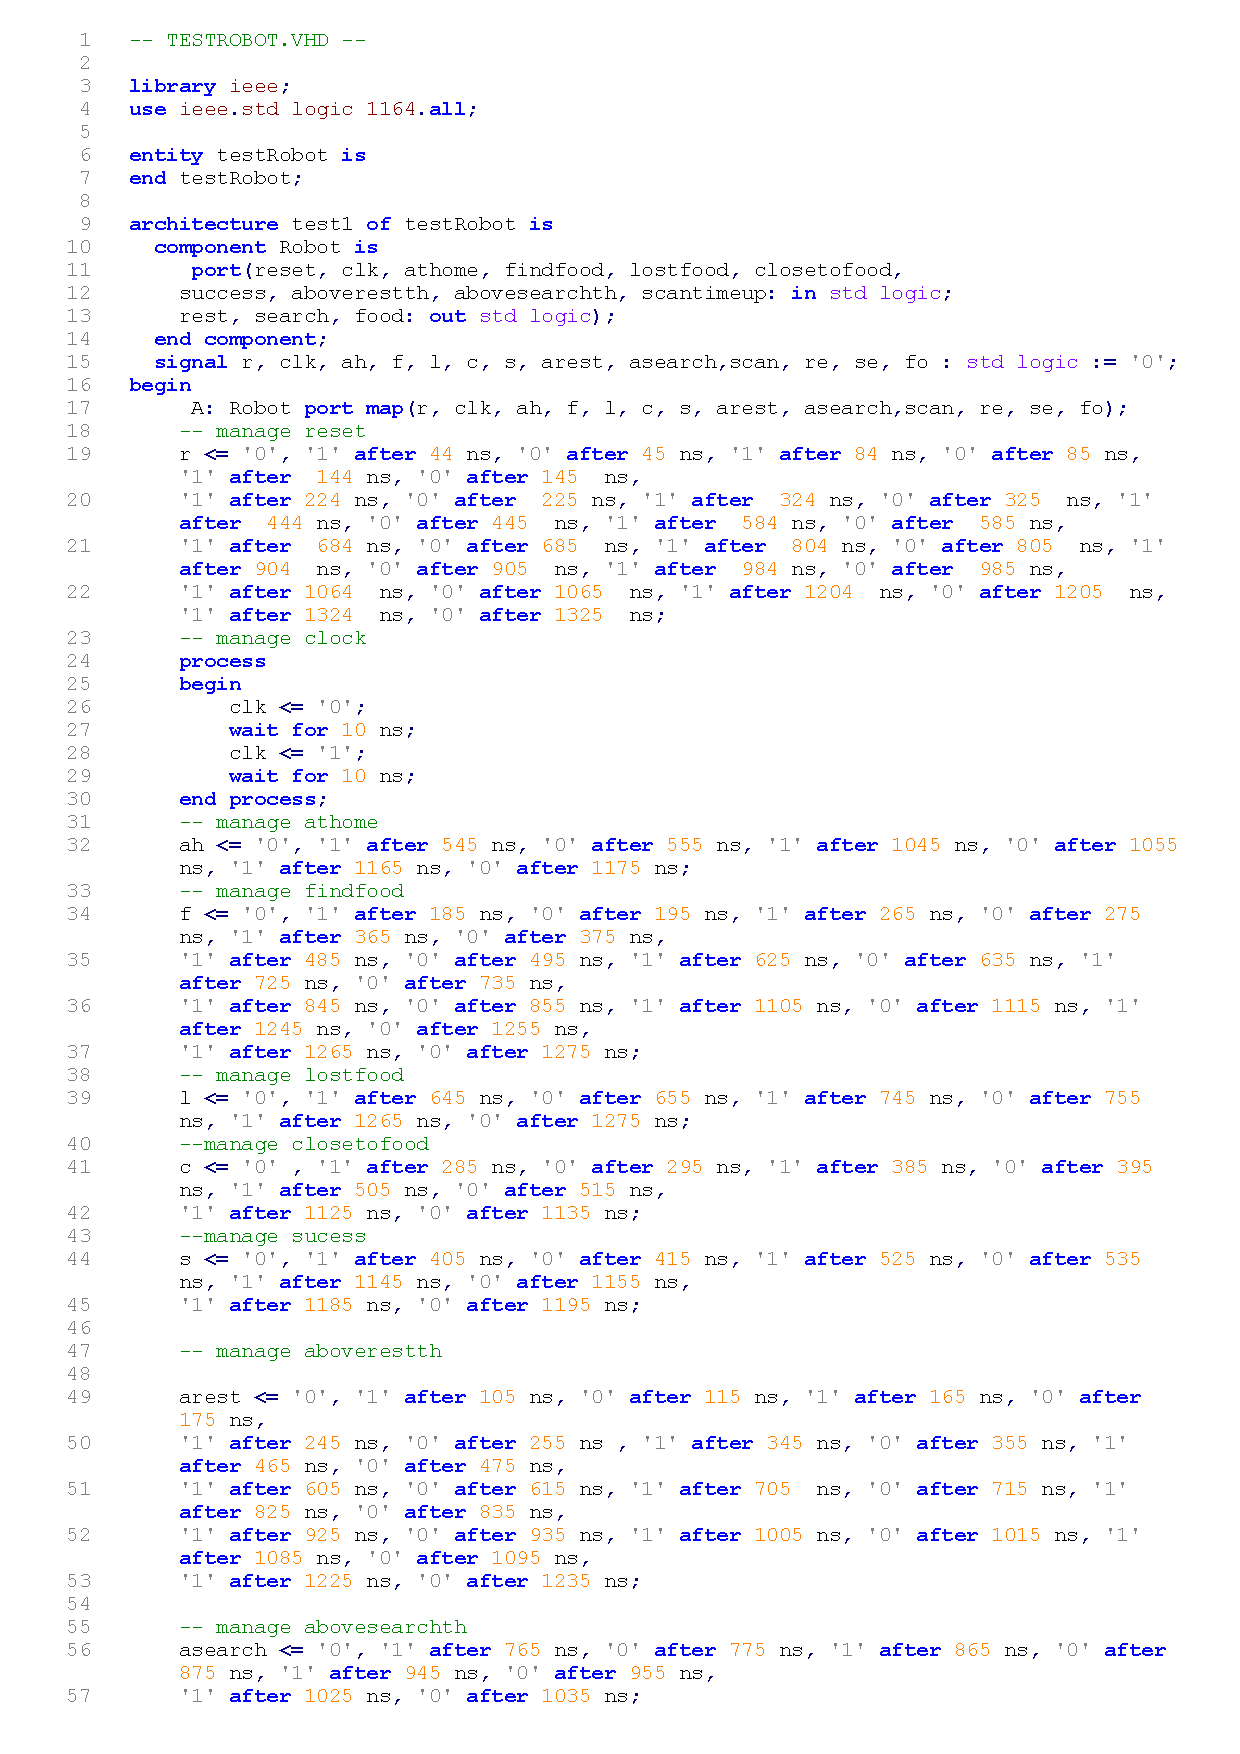
\includepdf{TestRobot.pdf}
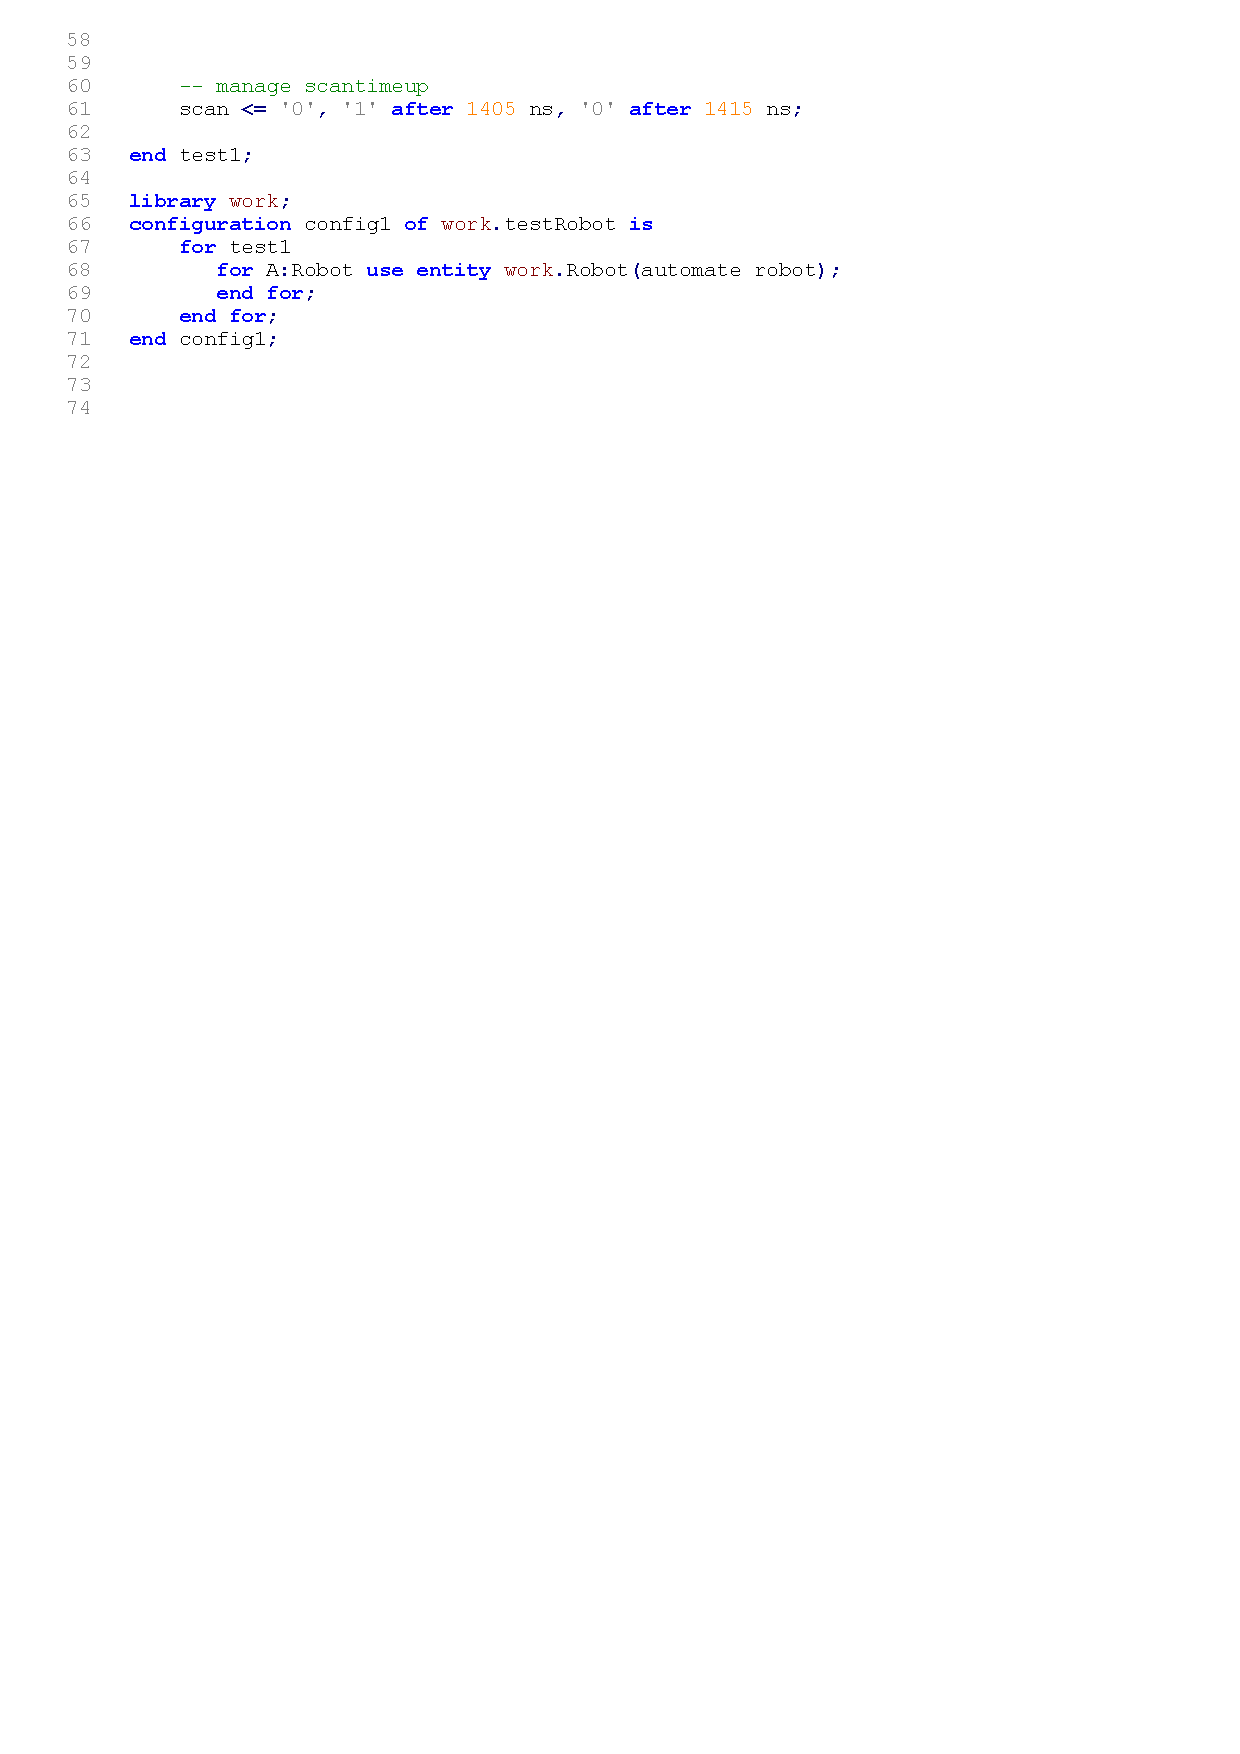
\includepdf{TestRobot2.pdf}
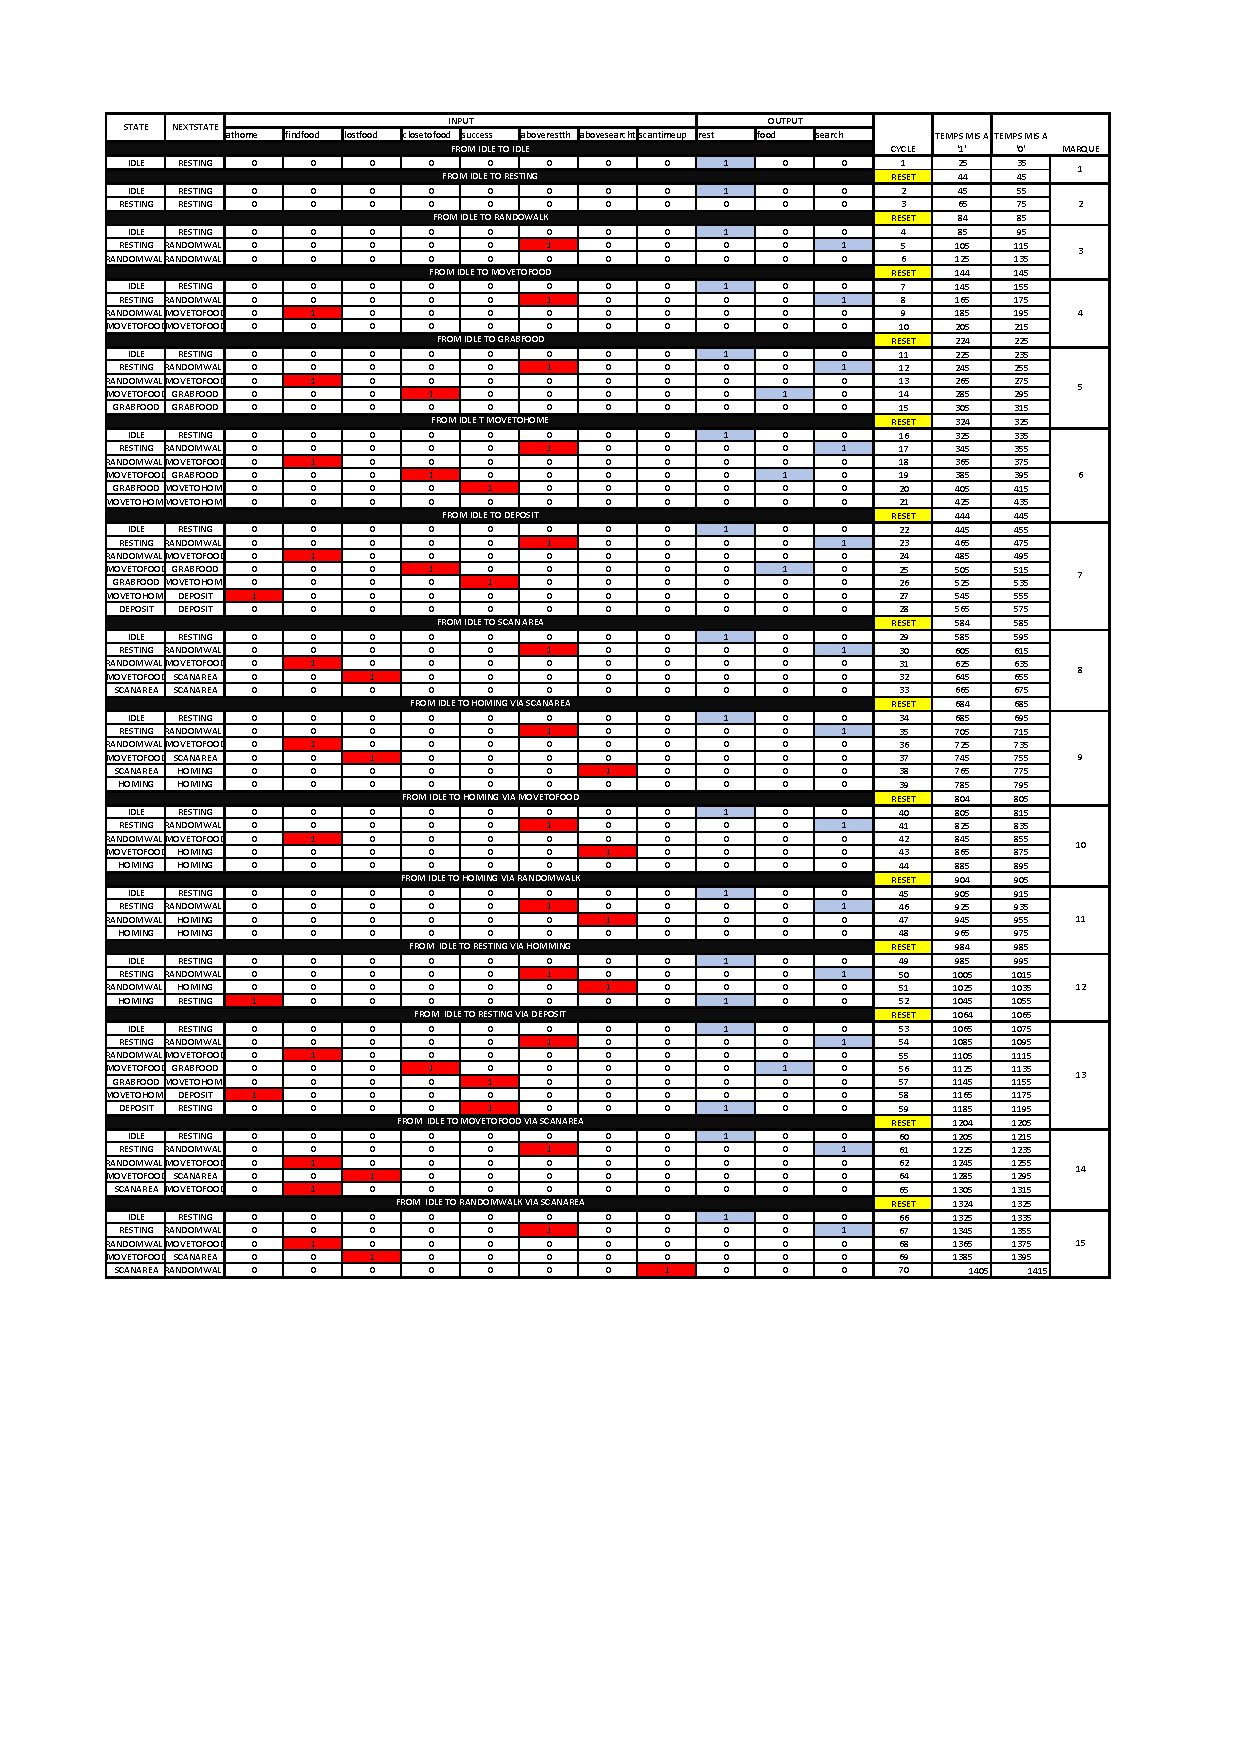
\includepdf{TestBench.pdf}
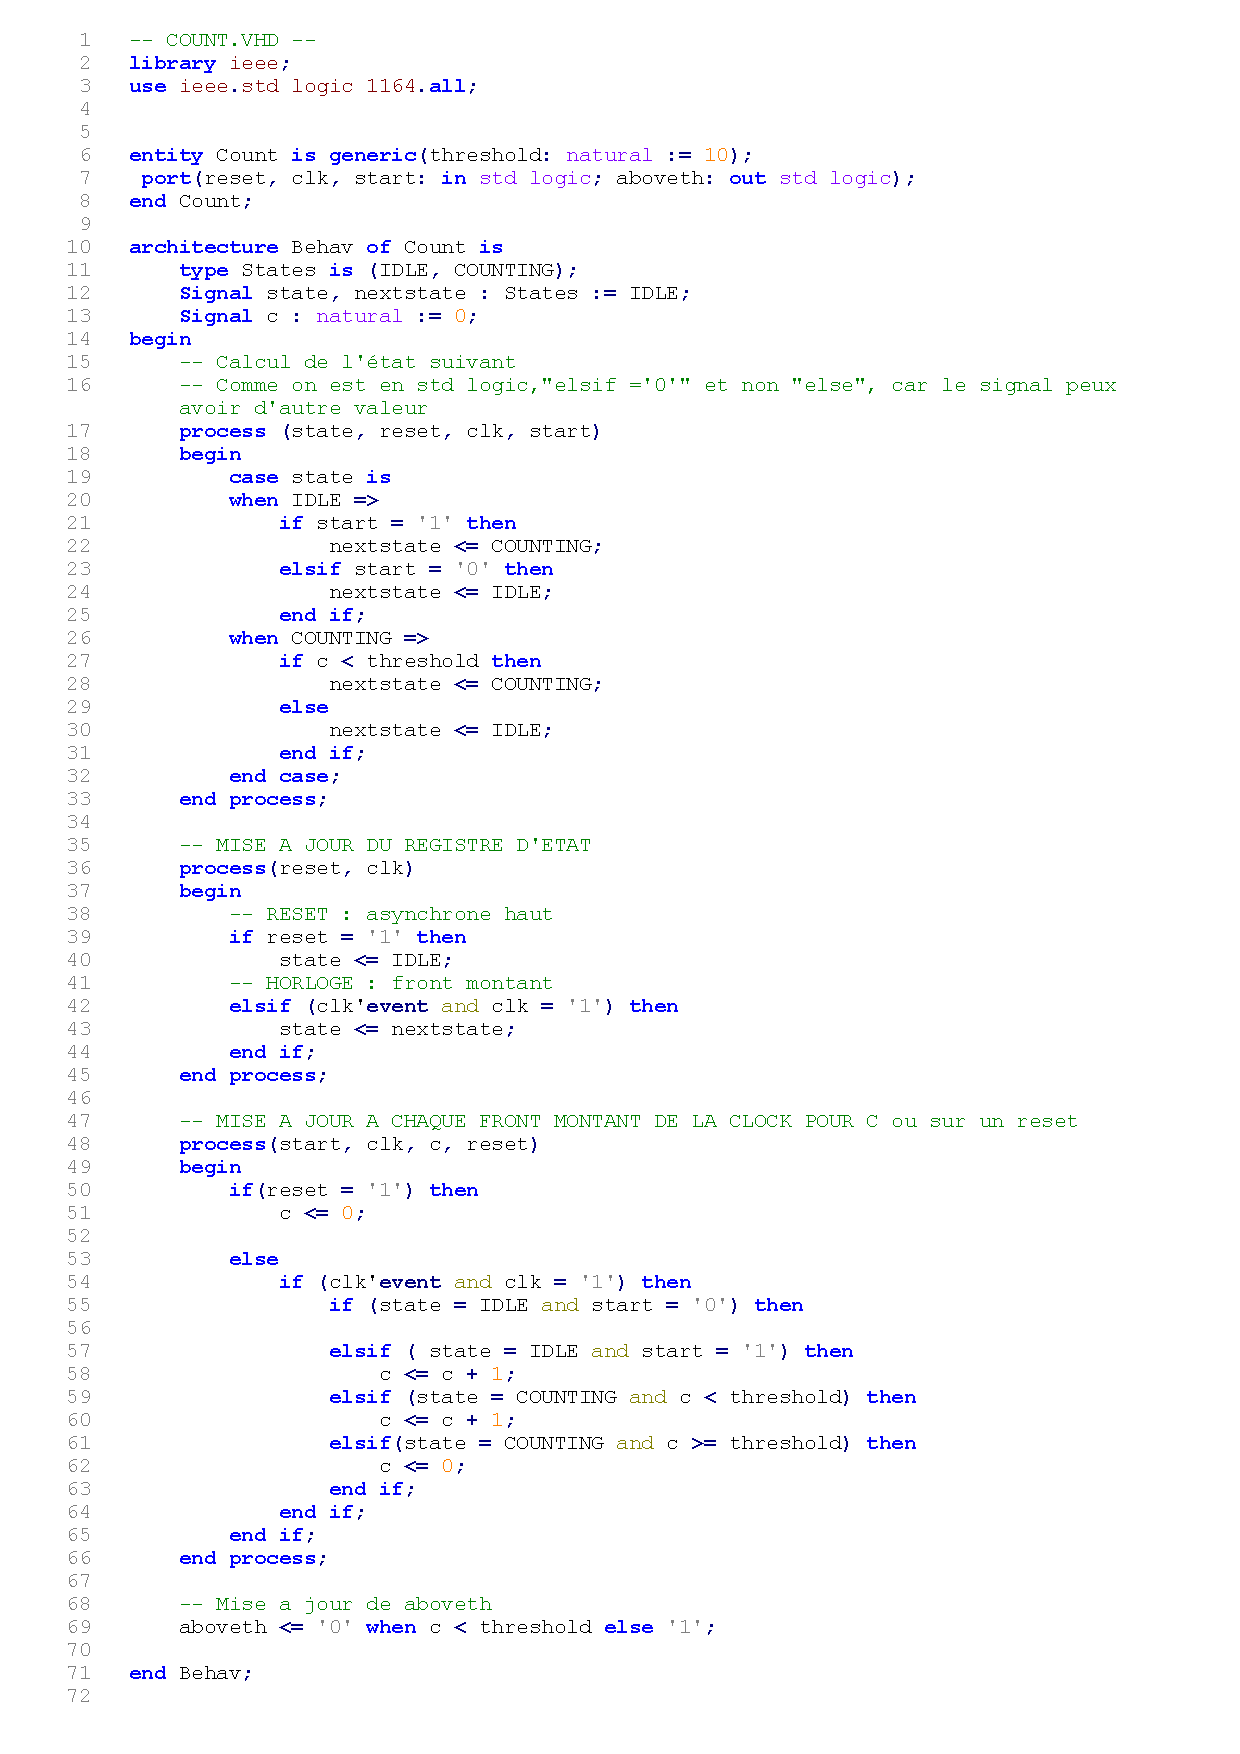
\includepdf{count.pdf}
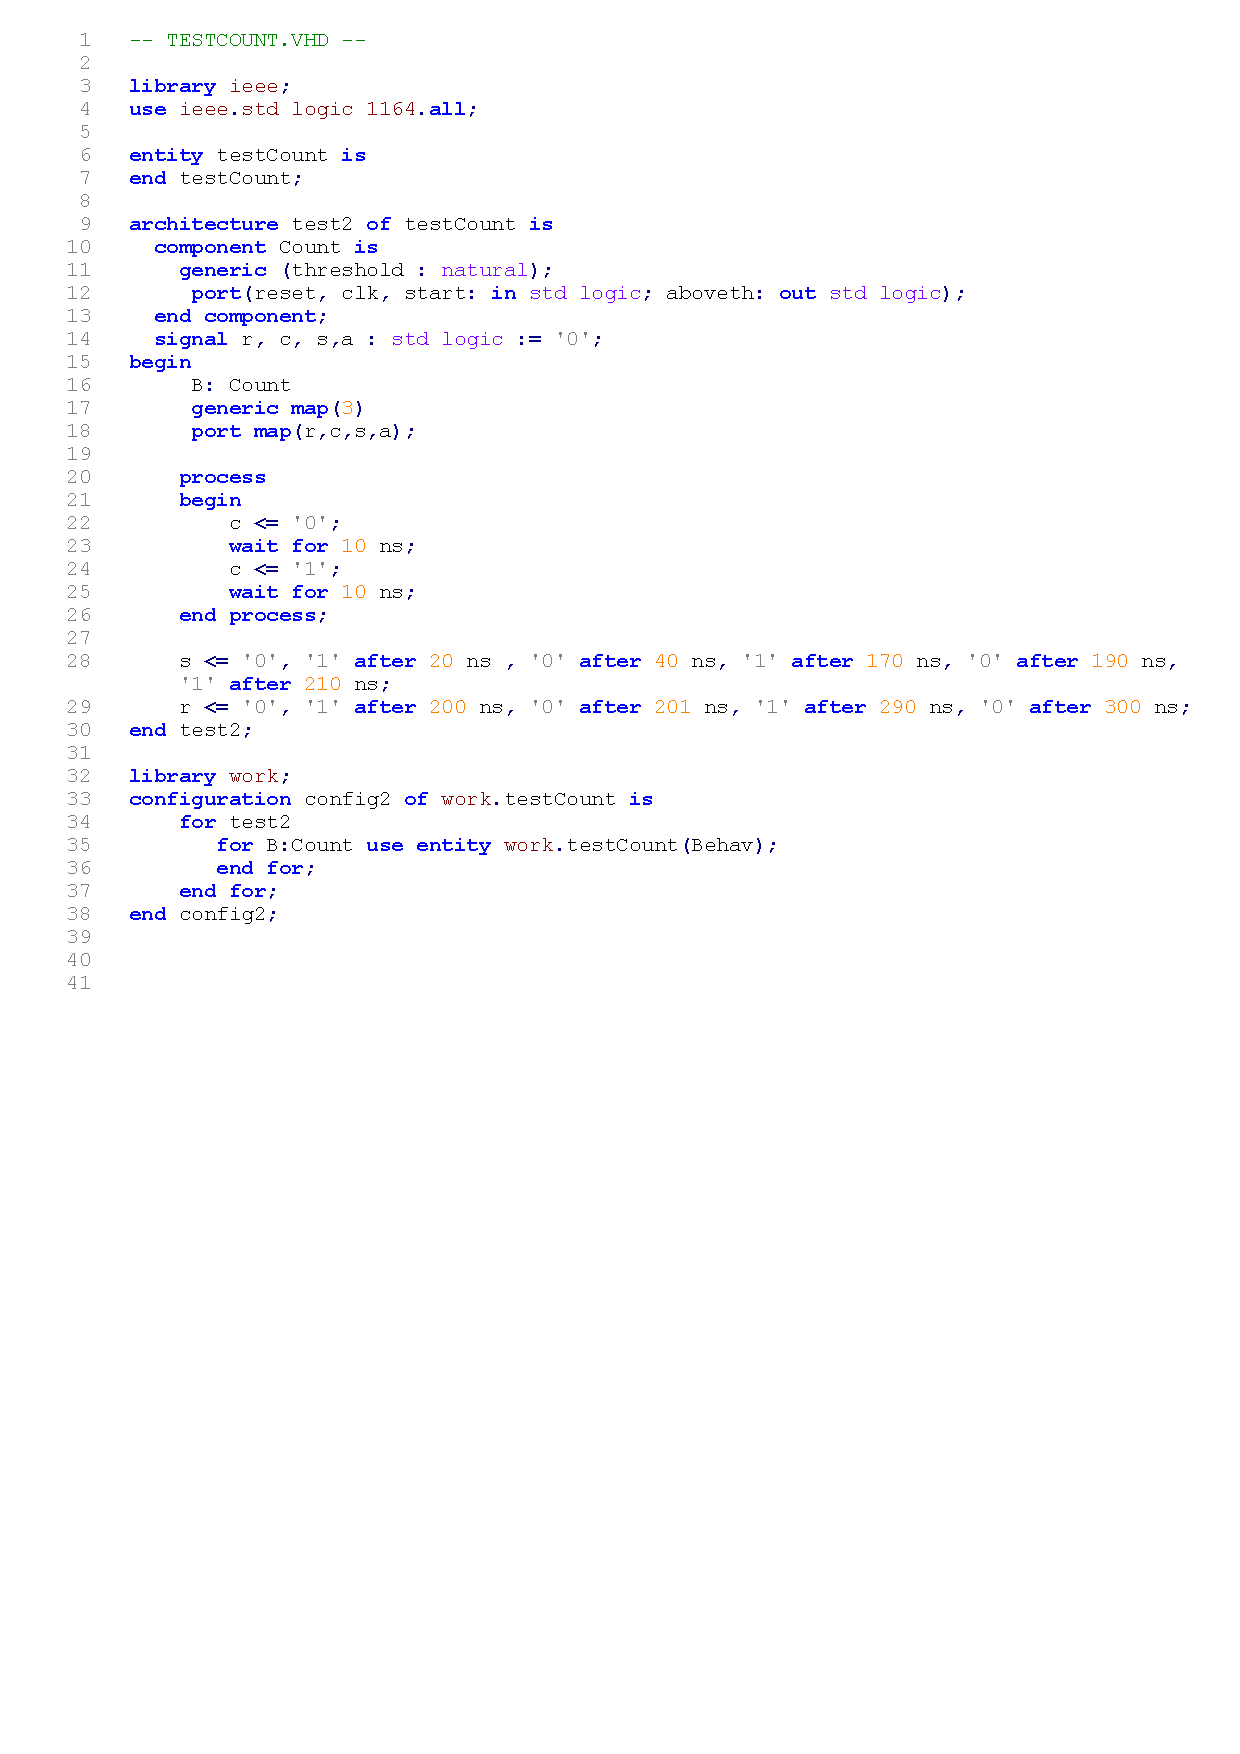
\includepdf{TestCount.pdf}

\begin{figure}[h]
\advance\leftskip+6cm
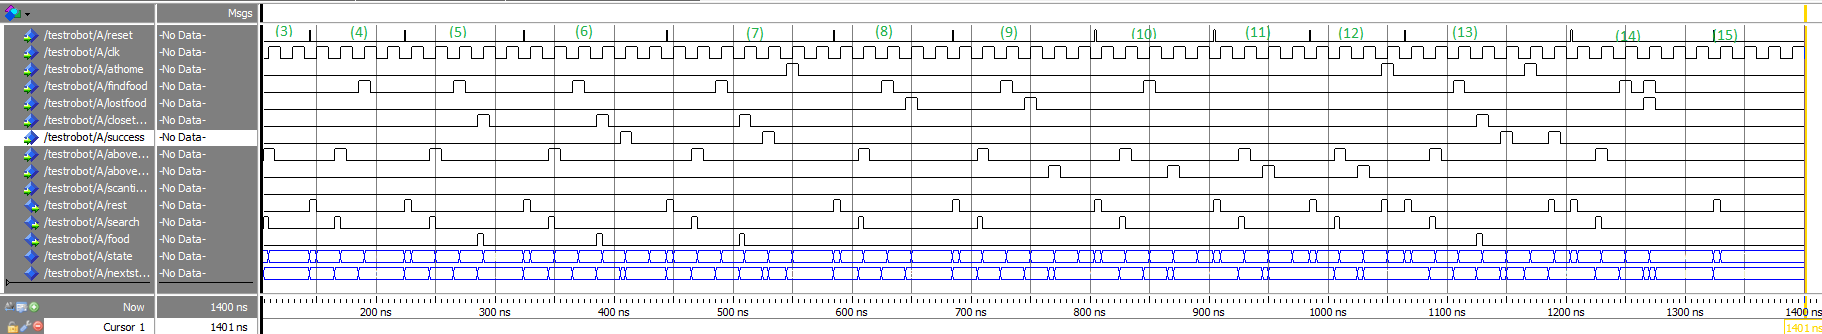
\includegraphics[scale=0.50, angle=-90]{TestRobotMain.PNG}
\caption{Simulation du robot}
\end{figure}

\begin{figure}[h]
\advance\leftskip+6cm
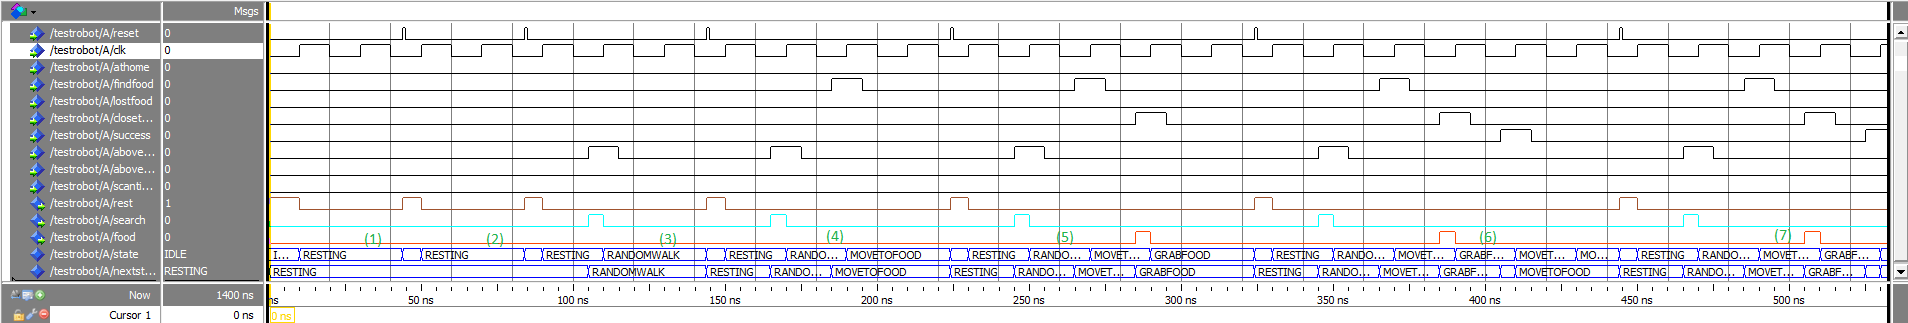
\includegraphics[scale=0.50, angle=-90]{detail_part1.PNG}
\caption{Simulation du robot : 0 ns à 500 ns}
\end{figure}

\begin{figure}[h]
\advance\leftskip+6cm
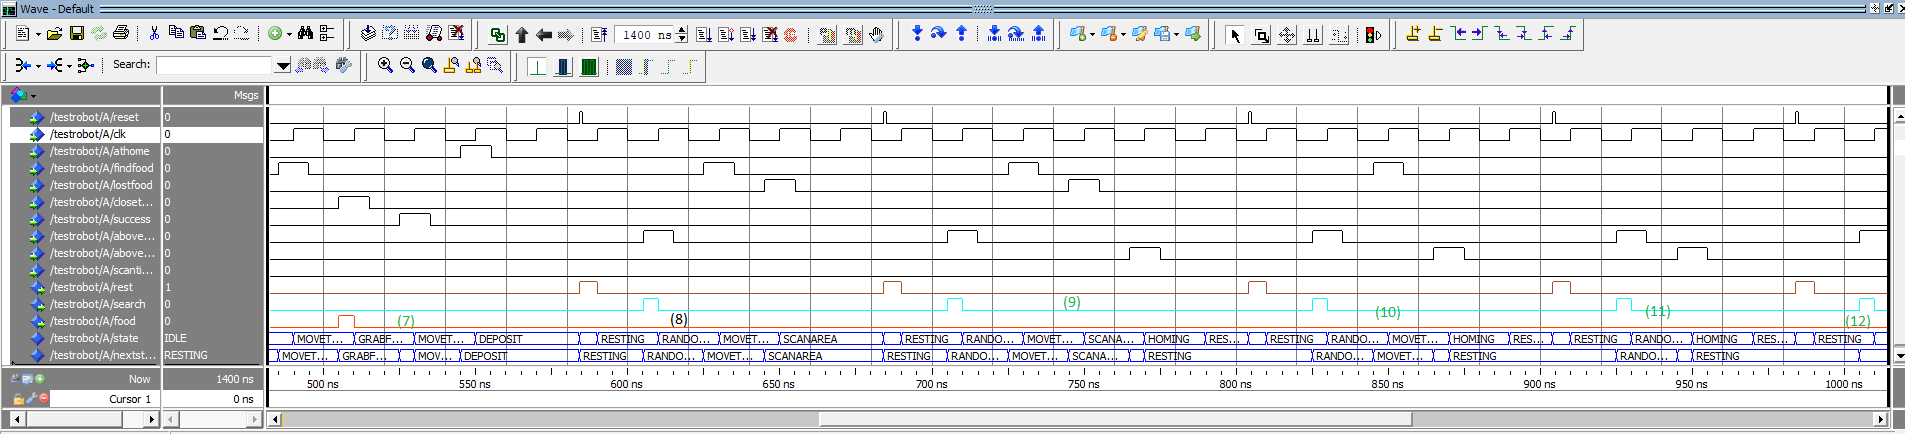
\includegraphics[scale=0.50, angle=-90]{detail_part2.PNG}
\caption{Simulation du robot : 500 ns à 1000 ns}
\end{figure}

\begin{figure}[h]
\advance\leftskip+6cm
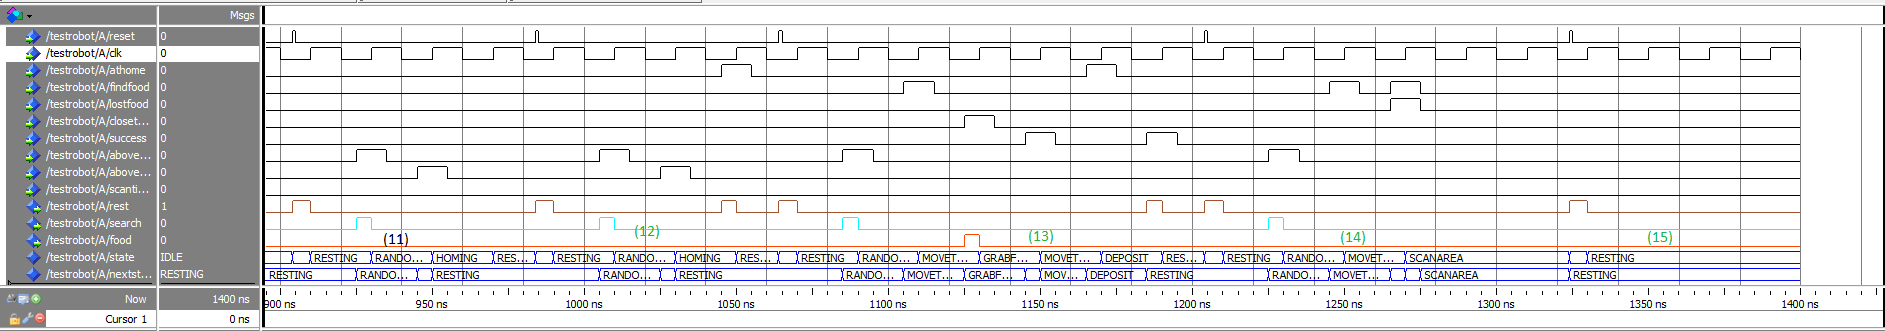
\includegraphics[scale=0.50, angle=-90]{detail_part3.PNG}
\caption{Simulation du robot : 1000 ns à 1500 ns}
\end{figure}

\begin{figure}[h]
\advance\leftskip+6cm
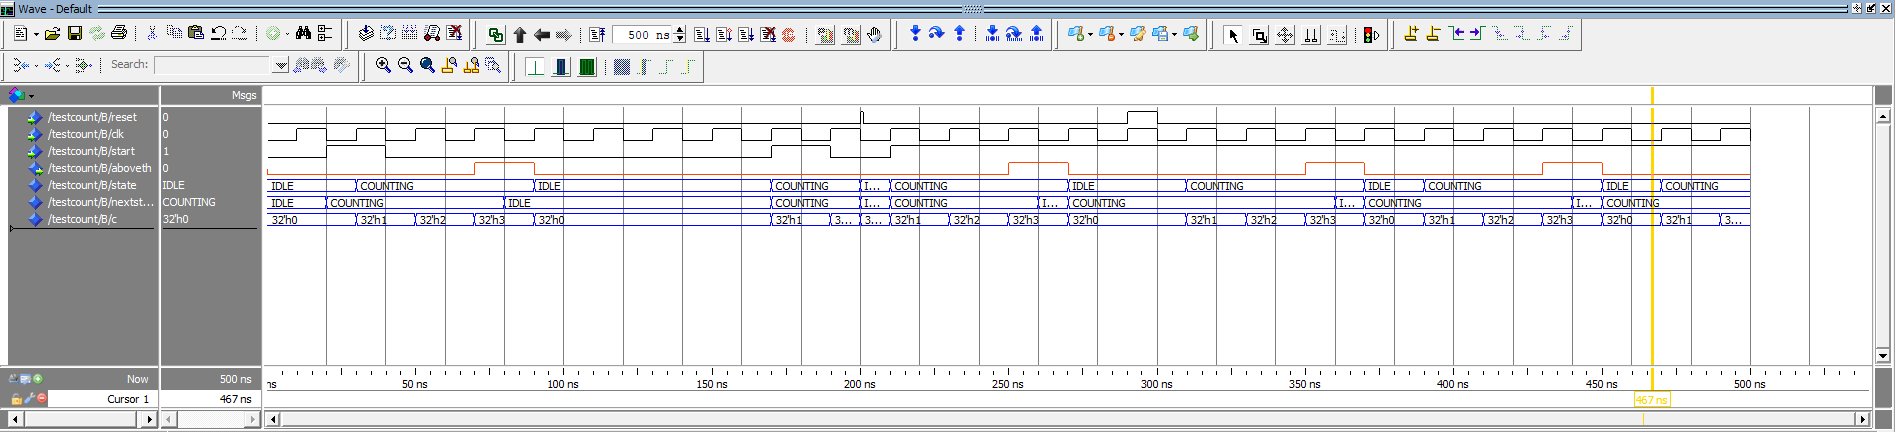
\includegraphics[scale=0.50, angle=-90]{count.PNG}
\caption{Simulation du Count}
\end{figure}

\end{document}